\documentclass{../notes}

\title{商务智能 HW04}

\loadgeometry{word-moderate}

\begin{document}
    \maketitle

    展开后的RNN结构如图\ref{fig:rnn-structure}所示:

    \begin{figure}[ht]
        \centering
        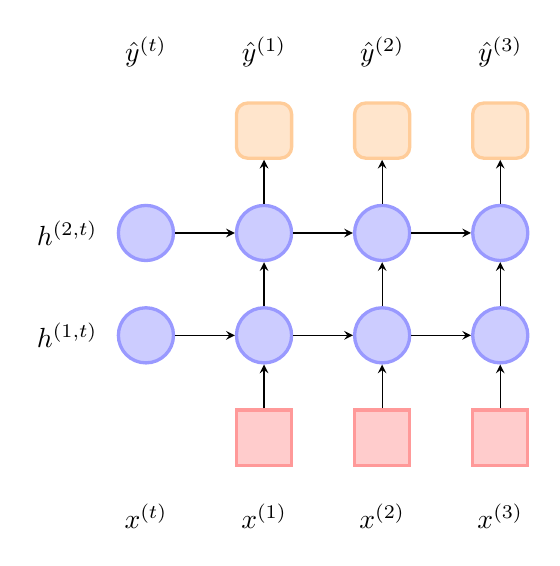
\begin{tikzpicture}
            [
                InputNode/.style={rectangle, draw=red!40, fill=red!20, very thick, minimum size = 7mm},
                HiddenNode/.style={circle, draw=blue!40, fill=blue!20, very thick, minimum size = 7mm},
                OutputNode/.style={rectangle, rounded corners, draw=orange!40, fill=orange!20, very thick, minimum size = 7mm},
                Connection/.style={-stealth}
            ]
            \node (Hidden_00){};
            \node [below of=Hidden_00]{$\bs x^{(t)}$};
            \foreach \t [evaluate=\t as \p using int(\t-1)] in {1, 2, 3} {
                \node[InputNode, right of=Hidden_0\p, xshift=0.5cm] (Hidden_0\t){};
                \node[below of=Hidden_0\t]{$\bs x^{(\t)}$};
            }
            \foreach \l [evaluate=\l as \p using int(\l-1)] in {1, 2} {
                \foreach \t in {0, 1, 2, 3} {
                    \node[HiddenNode, above of=Hidden_\p\t, yshift=0.3cm] (Hidden_\l\t) {};
                }
                \foreach \t [evaluate=\t as \n using int(\t+1)] in {0, 1, 2} {
                    \draw[Connection] (Hidden_\l\t) -> (Hidden_\l\n);
                }
                \node [left of=Hidden_\l0]{$\bs h^{(\l, t)}$};
            }
            \node [above of=Hidden_20, yshift=0.3cm](Hidden_30){};
            \node [above of=Hidden_30]{$\hat {\bs y}^{(t)}$};
            \foreach \t in {1, 2, 3} {
                \node[OutputNode, above of=Hidden_2\t, yshift=0.3cm] (Hidden_3\t){};
                \node[above of=Hidden_3\t]{$\hat {\bs y}^{(\t)}$};
                \foreach \l [evaluate=\l as \n using int(\l + 1)] in {0, 1, 2} {
                    \draw[Connection] (Hidden_\l\t) -> (Hidden_\n\t);
                }
            }
        \end{tikzpicture}
        \caption{展开后的RNN结构}
        \label{fig:rnn-structure}
    \end{figure}

    不考虑输入批次,令$\bs x^{(i)}, i=1,2,3$为列向量。设隐藏层$i$的输入权重为、循环权重分别为$\bs W^{(i)}_i, \bs W^{(i)}_h$,输入偏置、循环偏置分别为$\bs b^{(i)}_i, \bs b^{(i)}_h$,令$\bs b^{(i)} = \bs b^{(i)}_i + \bs b^{(i)}_h$。激活函数为$f(\cdot)$。

    计算两层RNN的输出如表\ref{tbl:rnn-result-1}:

    \begin{table}[ht]
        \centering
        \small
        \caption{两层RNN的输出}
        \begin{tabular}{cccc}
            \toprule
            & $t = 1$ & $t = 2$ & $t = 3$ \\
            \midrule
            第1层 & $f\left(\bs W^{(1)}_i \bs x^{(1)} + \bs W^{(1)}_h \bs h^{(1, 0)} + \bs b^{(1)}\right) $ & $f\left(\bs W^{(1)}_i \bs x^{(2)} + \bs W^{(1)}_h \bs h^{(1, 1)} + \bs b^{(1)}\right) $ & $f\left(\bs W^{(1)}_i \bs x^{(3)} + \bs W^{(1)}_h \bs h^{(1, 2)} + \bs b^{(1)}\right)$ \\
            第2层 & $f\left(\bs W^{(2)}_i \bs h^{(1, 1)} + \bs W^{(2)}_h \bs h^{(2, 0)} + \bs b^{(2)}\right)$ & $f\left(\bs W^{(2)}_i \bs h^{(1, 2)} + \bs W^{(2)}_h \bs h^{(2, 1)} + \bs b^{(1)}\right)$ & $f\left(\bs W^{(2)}_i \bs h^{(1, 3)} + \bs W^{(2)}_h \bs h^{(2, 2)} + \bs b^{(2)}\right)$ \\
            \bottomrule
        \end{tabular}
        \label{tbl:rnn-result-1}
    \end{table}
\end{document}